\section[The \Dumux Models]{Physical and Numerical Models Available in \Dumux}
\todo[inline]{Evtl. könnten wir das in zwei kapitel aufsplitten? Physical und numerical
 models}

\subsection{Physical and Mathematical Description}

Characteristic of compositional multiphase models is that the phases
are not only matter of a single chemical substance. Instead, their
composition in general includes several species, and for the mass transfer,
the component behavior is quite different from the phase behavior. In the following, we
give some basic definitions and assumptions that are required for the
formulation of the model concept below. As an example, we take a
three-phase three-component system water-NAPL-gas
\cite{A3:class:2002a}. The modification for other multicomponent
systems is straightforward and can be found, e.\ g., in
\cite{A3:bielinski:2006,A3:acosta:2006}.

\subsubsection{Basic Definitions and Assumptions for the Compositional
  Model Concept}
\textbf{Components:}
The term {\it component} stands for constituents of the phases which
can be associated with a unique chemical species, or, more generally, with
a group of species exploiting similar physical behavior. In this work, we
assume a water-gas-NAPL system composed of the phases water (subscript
$\text{w}$), gas ($\text{g}$), and NAPL ($\text{n}$). These phases are
composed of the components water (superscript $\text{w}$), air
($\text{a}$), and the organic contaminant ($\text{c}$) (see Fig.\
\ref{fig:phaseMassEnergyTransfer}).

\begin{figure}
  \centering
  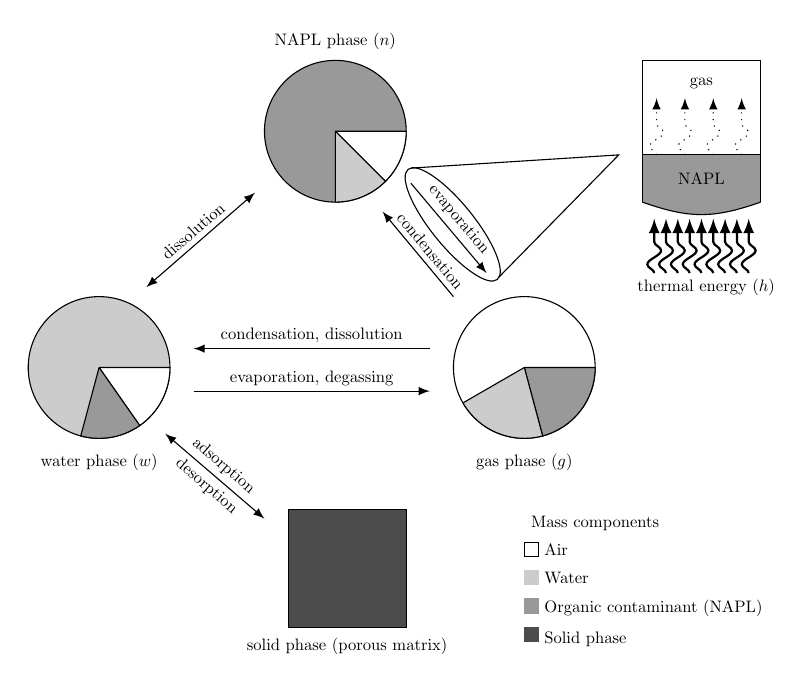
\begin{tikzpicture} [>=latex,scale=0.6, every node/.style={transform shape}]
    % Ellipse 1 solid
    \coordinate (A) at (1,-0.5);
    \draw [fill=black!70](A) rectangle(3.5,2) node at(2.25,-0.9) {solid phase (porous matrix)};
    % Ellipse 2 water
    \coordinate (B) at (-3,5);
    \draw [fill=black!20](B) circle(1.5cm);
    \node [yshift=5mm]at(-3,2.5){water phase $(w)$};
    \draw[fill=white] (B)--+(1.5,0)arc(0:-55:1.5cm)--(B);
    \draw[fill=black!40] (B)--+(-55:1.5cm)arc(-55:-105:1.5cm)--(B);
    % Ellipse 3 gas
    \coordinate (C) at (6,5);
    \draw [](C) circle (1.5cm);
    \node[yshift=5mm]at(6,2.5){gas phase $(g)$};
    \draw [fill=black!40](C)--+(1.5,0)arc(0:-75:1.5cm)--(C);
    \draw [fill=black!20] (C)--+(-75:1.5cm)arc(-75:-150:1.5cm)--(C);
    % Ellipse 4 napl
    \coordinate (D) at (2,10);
    \draw [fill=black!40](D) circle (1.5cm);
    \node[yshift=5mm]at(2,11.4){NAPL phase $(n)$};
    \draw [fill=white](D)--+(1.5,0)arc(0:-45:1.5cm)--(D);
    \draw [fill=black!20] (D)--+(0,-1.5)arc(-90:-45:1.5cm)--(D);
    % arrows
    %A-B
      \draw [<->,white](0.5,1.8)--(-1.6,3.6) node[black,above,sloped,pos=0.5]{adsorption};
      \draw [<->](0.5,1.8)--(-1.6,3.6) node[below,sloped,pos=0.5]{desorption};
    %B-C
      \draw[<-](-1,5.4)--(4,5.4)node[above,sloped,pos=0.5]{condensation, dissolution};
      \draw[->](-1,4.5)--(4,4.5)node[above,sloped,pos=0.5]{evaporation, degassing};
    %B-D
      \draw[<->](-2,6.7)--(0.3,8.7)node[above,sloped,pos=0.5]{dissolution};
    %D-C
      \draw[->](3.6,8.9)--(5.2,7)node[above,sloped,pos=0.5]{evaporation};
      \draw[rotate around={-51:(4,6.8)}](3.35,7.95) ellipse (1.5cm and 0.45cm);  %Ellipse um evaporation
      \draw (3.6,9.22)--(8,9.5)--(5.45,6.9);
      \draw[<-](3,8.3)--(4.5,6.5)node[above,sloped,pos=0.55]{condensation};
    % thermal energy
    \filldraw [black!40](8.5,9.5)rectangle(11,8.5);
    \draw (8.5,9.5)rectangle(11,11.5);
    \draw (8.5,9.5)--(8.5,8.5);
    \draw (11,9.5)--(11,8.5);
    \draw [decorate,decoration={bent,aspect=0.4,amplitude=6},fill=black!40](11,8.5)--(8.5,8.5);
    \foreach \x in {8.75,9,...,10.8}
    \draw [->,decorate,decoration={snake,post length=2mm},thick](\x,7)--(\x,8.15);
    \foreach \x in {8.8,9.4,10,10.6}
    \draw [->,dotted,decorate,decoration={snake,post length=2mm}](\x,9.5)--(\x,10.7);
    \node at(9.75,11){gas};
    \node at(9.75,9){NAPL};
    \node at(9.85,6.7){thermal energy $(h)$};
    % legende
    \node at (7.5,1.7){Mass components};
    \draw[](6,1)rectangle +(0.3,0.3) node at(6.3,1.15) [right]{Air};
    \filldraw[black!20](6,0.4) rectangle +(0.3,0.3) node at (6.3,0.55)[black,right]{Water};
    \filldraw[black!40](6,-0.2) rectangle +(0.3,0.3) node at (6.3,-0.1)[right,black]{Organic contaminant (NAPL)};
    \filldraw[black!70](6,-0.8) rectangle +(0.3,0.3) node at (6.3,-0.75)[right,black]{Solid phase};
  \end{tikzpicture}
  \caption{Mass and energy transfer between the phases}
  \label{fig:phaseMassEnergyTransfer}
\end{figure}

\textbf{Equilibrium:}
For the non-isothermal multiphase processes in porous media under
consideration, we state that the assumption of local thermal
equilibrium is valid since flow velocities are small. We neglect
chemical reactions and biological decomposition and assume chemical
equilibrium.  Mechanical equilibrium is not valid in a porous medium,
since discontinuities in pressure can occur across a fluid-fluid
interface due to capillary effects.

\textbf{Notation:} The index $\alpha \in \{\text{w}, \text{n}, \text{g}\}$ refers
to the phase, while the superscript $\kappa \in \{\text{w}, \text{a}, \text{c}\}$ refers
to the component. \\
\begin{tabular}{llll}
$p_\alpha$ & phase pressure & $\phi$ & porosity \\
$T$ & temperature & $K$ & absolute permeability tensor \\
$S_\alpha$ & phase saturation & $\tau$ & tortuosity \\
$x_\alpha^\kappa$ & mole fraction of component $\kappa$ in phase $\alpha$ & $\boldsymbol{g}$ & gravitational acceleration \\
$X_\alpha^\kappa$ & mass fraction of component $\kappa$ in phase $\alpha$ & $q^\kappa_\alpha$ & volume source term of $\kappa$ in $\alpha$ \\
$\varrho_{\text{mol},\alpha}$ & molar density of phase $\alpha$ & $u_\alpha$ & specific internal energy \\
$\varrho_{\alpha}$ & mass density of phase $\alpha$ & $h_\alpha$ & specific enthalpy \\
$M$ & molar mass of a phase or component & $c_\text{s}$ & specific heat enthalpy \\
$k_{\text{r}\alpha}$ & relative permeability & $\lambda_\text{pm}$ & heat conductivity \\
$\mu_\alpha$ & phase viscosity & $q^h$ & heat source term \\
$D_\alpha^\kappa$ & diffusivity of component $\kappa$ in phase $\alpha$ & $\boldsymbol{v}_{a,\alpha}$  & advective velocity \\
$\boldsymbol{v}_\alpha$ & velocity (Darcy or free flow)& & \\
\end{tabular}


\subsubsection{Balance Equations}
For the balance equations for multicomponent systems, it is in many
cases convenient to use a molar formulation of the continuity
equation. Considering the mass conservation for each component allows
us to drop source/sink terms for describing the mass transfer between
phases. Then, the
molar mass balance can be written as:
%
\begin{multline}
  \label{A3:eqmass1}
 \phi \frac{\partial (\sum_\alpha \varrho_{\text{mol}, \alpha}
    x_\alpha^\kappa S_\alpha )}{\partial t}
 - \sum\limits_\alpha \Div \left\lbrace \frac{k_{\text{r}
        \alpha}}{\mu_\alpha} \varrho_{\text{mol}, \alpha}
    x_\alpha^\kappa \textbf{K} (\grad p_\alpha -
    \varrho_{\alpha} \boldsymbol{g}) \right\rbrace  \\
  %
  %
 - \sum\limits_\alpha \Div \left\lbrace \tau \phi S_\alpha D_\alpha^\kappa \varrho_{\text{mol},
      \alpha} \grad x_\alpha^\kappa \right\rbrace
 - q^\kappa = 0, \qquad \kappa \in \{\text{w,a,c}\}.
\end{multline}

The component mass balance can also be written in terms of mass fractions
by replacing molar densities by mass densities and mole by mass fractions.
To obtain a single conserved quantity in the temporal derivative, the total
concentration, representing the mass of one component per unit volume, is defined as
\begin{displaymath}
C^\kappa = \sum_\alpha \phi S_\alpha \varrho_{\text{mass},\alpha} X_\alpha^\kappa \; .
\end{displaymath}
Using this definition, the component mass balance is written as:

\begin{multline}
  \label{A3:eqmass2}
    \frac{\partial C^\kappa}{\partial t} =
  \sum\limits_\alpha \Div \left\lbrace \frac{k_{\text{r}
        \alpha}}{\mu_\alpha} \varrho_{\text{mass}, \alpha}
    X_\alpha^\kappa \textbf{K} (\grad p_\alpha +
    \varrho_{\text{mass}, \alpha} \boldsymbol{g}) \right\rbrace  \\
  %
  %
   + \sum\limits_\alpha \Div \left\lbrace \tau \phi S_\alpha D_\alpha^\kappa \varrho_{\text{mass},
      \alpha} \frac{M^\kappa}{M_\alpha} \grad x_\alpha^\kappa \right\rbrace
 + q^\kappa = 0, \qquad \kappa \in \{\text{w,a,c}\}.
\end{multline}


In the case of non-isothermal systems, we further have to balance the
thermal energy. We assume fully reversible processes, such that entropy
is not needed as a model parameter. Furthermore, we neglect
dissipative effects and the heat transport due to molecular
diffusion. The energy balance can then be
formulated as:
%
\begin{multline}
  \label{A3:eqenergmak1}
  \phi \frac{\partial \left( \sum_\alpha \varrho_{\alpha}
      u_\alpha S_\alpha \right)}{\partial t} + \left( 1 -
    \phi \right) \frac{\partial \varrho_{\text{s}} c_{\text{s}}
    T}{\partial t}
 - \Div \left( \lambda_{\text{pm}} \grad T \right)
   \\
   - \sum\limits_\alpha \Div \left\lbrace \frac{k_{\text{r}
        \alpha}}{\mu_\alpha} \varrho_{\alpha} h_\alpha
    K \left( \grad p_\alpha - \varrho_{\alpha}
      \boldsymbol{g} \right) \right\rbrace
 - q^h \; = \; 0.
\end{multline}

In order to close the system, supplementary constraints for capillary pressure, saturations and mole
fractions are needed, \cite{A3:helmig:1997}.
According to the Gibbsian phase rule, the number of degrees of freedom
in a non-isothermal compositional multiphase system is equal to the
number of components plus one. This means we need as many independent
unknowns in the system description. The
available primary variables are, e.\ g., saturations, mole/mass
fractions, temperature, pressures, etc.

\subsection{Available Models}
The following description of the available models is automatically extracted
from the Doxygen documentation.

\todo[inline]{Die Modelle waren etwas uneinheitlich von der Notation (ich habe
  hier auch gerade das entsprechende ToDo entfernt). Das ist naturlich jetzt
  nicht mehr so schlimm, da die Modelle nicht mehr untereinander auftauchen,
  allerdings wird auch die Fehlersuche schwieriger (aus dem Auge aus dem Sinn).}

\todo[inline]{evtl. entferne Unterkapitel. Einfugen der Modelliste, die könnte
  in ahnlicher Form auch aufs doxygen? Update der Liste in die Release Manager
  Tasks ubernehmen}

\subsubsection{Fully-Implicit Models}

The fully-implicit models described in this section are using the box or the
cell centered finite volume method as described in section \ref{box} and \ref{cc}
for spatial and the implicit Euler
method as temporal discretization. The models themselves are located in
subdirectories of \texttt{dumux/implicit} of the \Dumux distribution.

\subsubsection{Decoupled Models}
%
The basic idea the so-called decoupled models have in common is to reformulate the
equations of multi-phase flow (e.g. Eq. \ref{A3:eqmass1}) into one equation for
pressure and equations for phase-/component-/etc. transport. The pressure equation
is the sum of the mass balance equations and thus considers the total flow of the
fluid system. The new set of equations is considered as decoupled (or weakly coupled)
and can thus be solved sequentially. The most popular decoupled model is the so-called
fractional flow formulation for two-phase flow which is usually implemented applying
an IMplicit Pressure Explicit Saturation algorithm (IMPES).
In comparison to a fully implicit model, the decoupled structure allows the use of
different discretization methods for the different equations. The standard method
used in the decoupled models is a cell centered finite volume method. Further schemes,
so far only available for the two-phase pressure equation, are cell centered finite
volumes with multi-point flux approximation (MPFA O-method) and mimetic finite differences.

An $h$-adaptive implementation of both decoupled models is provided for two dimensions.
